\section{Постановка задачи и описание данных} \label{section:task}

\subsection{Неформальная постановка задачи}
Пусть имеется выборка трехмерных обектов, представленных в виде облаков точек (point clouds). Необходимо создать алгоритм, который на основе данной выборки будет генерировать \textit{новые} объекты подобные объектам в выборке, то есть будет генерировать новые объекты с сохранением статистических и геометрических свойств исходных объектов.

\subsection{Формальная постановка задачи}


\textit{Облако точек} - структура данных для представления геометрической формы некоторого объекта в виде неупорядоченного множества точек. Для трехмерного случая облаком точек будет называться неупорядоченное множество 
$P = \{(x_{i}, y_{i}, z_{i})\}_{i=1}^{N}$, где $N$ -- число точек в облаке.

Пусть у нас имеется выборка облаков точек подчиненных некоторому вероятностному распределению $p(X)$: $X_{1}, \ldots, X_{L} \sim p(X)$. Пусть распределение $q(X|z, \theta)$ аппроксимирует (оценивает, estimate) распределение $p$. Требуется построить алгоритм для семлирования объектов, подчиняющийся распределению $q$.

\subsection{Описание данных}

В данной работе, поставленная задача, изучается и решается на основе выборки зубов человека.

Опишем некоторые термины и понятия из зубного дела.

\subsubsection{Зубная анатомия}

Зубы классифицируются на резцы (incisors), клыки (canines), премоляры (premolars) и моляры (molars). Вместе зубы объединяются в верхний и нижний зубные ряды. Каждая зубная дуга (dental arch), или по-другому ряд зубов, разделяется на левую и правую часть. С каждой стороны у человека имеется два резца, один клык, два премоляра и три моляра \cite{kumar} см. рис. \ref{fig:dental_parts}.

\begin{figure}[h]
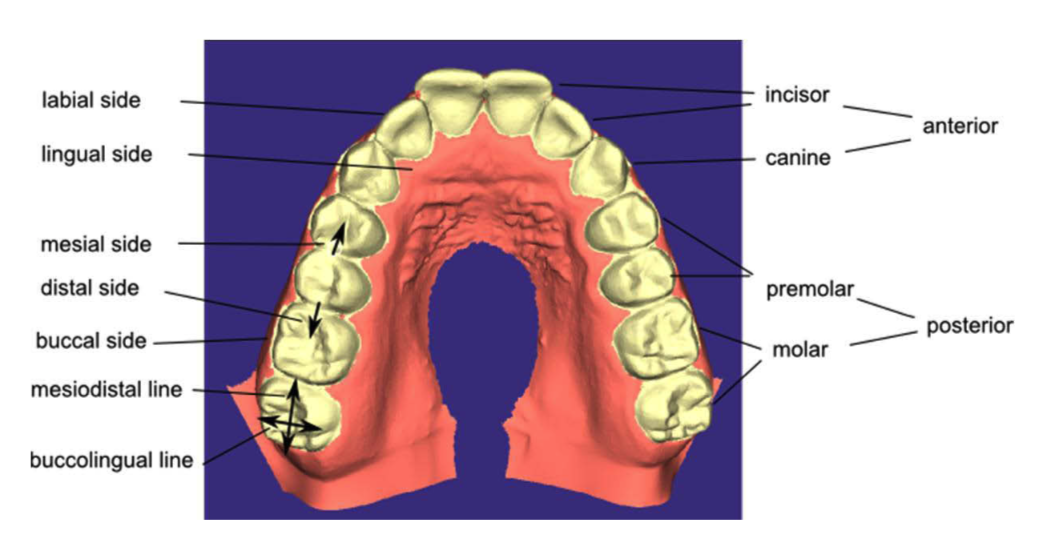
\includegraphics[width=1\linewidth]{images/dental_parts.png}
\caption{Анатомия зубов}
\label{fig:dental_parts}
\end{figure}

% ls | grep -e "^[0-9]" | while read dir; do ls $dir | nl | tail -n1; done

\subsubsection{Размер выборки}

В выборке присутствуют 28 типов зубов (все, кроме третьих моляров - зубов мудрости), для каждого типа зуба имеется от 124 до 150 экземпляров. Все экземпляры представлены в виде трехмерных сеток (перед началом работы основного алгоритма мы переводим их в облака точек, путем удаления ребер). Примеры экземпляров из выборки можно увидеть на  изображениях 2 - 7. %\ref{fig_ex1abc},  \ref{fig:ex2}, \ref{fig:ex3},  \ref{fig:ex4}, \ref{fig:ex5}. % 2 - 6


\begin{figure*}[ht!]
	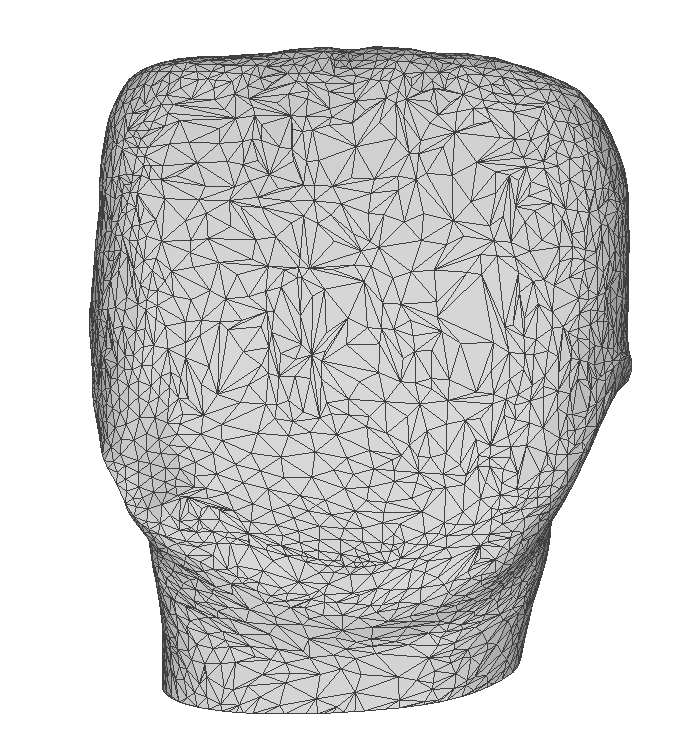
\includegraphics[width=.3\textwidth]{images/snapshot100.png}\hfill
    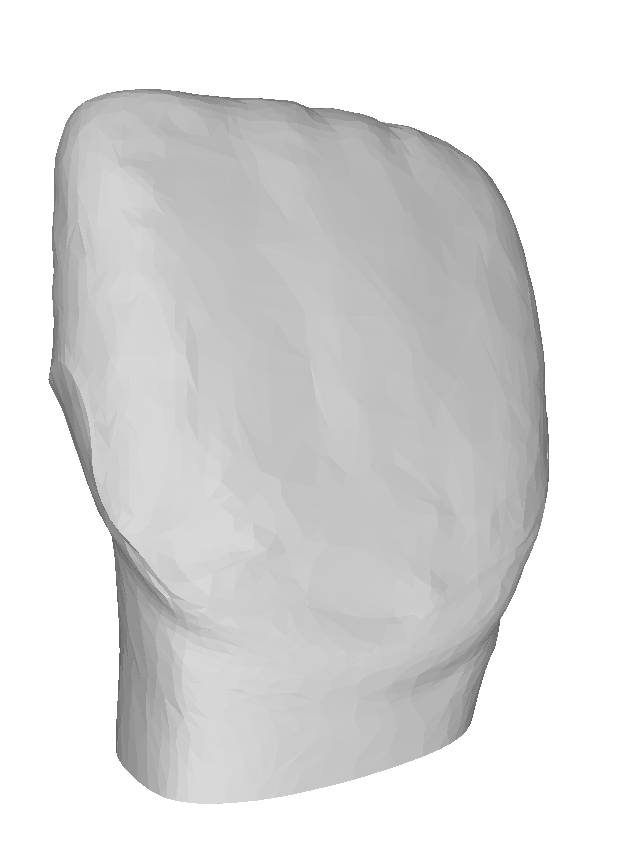
\includegraphics[width=.3\textwidth]{images/snapshot101.png}\hfill
    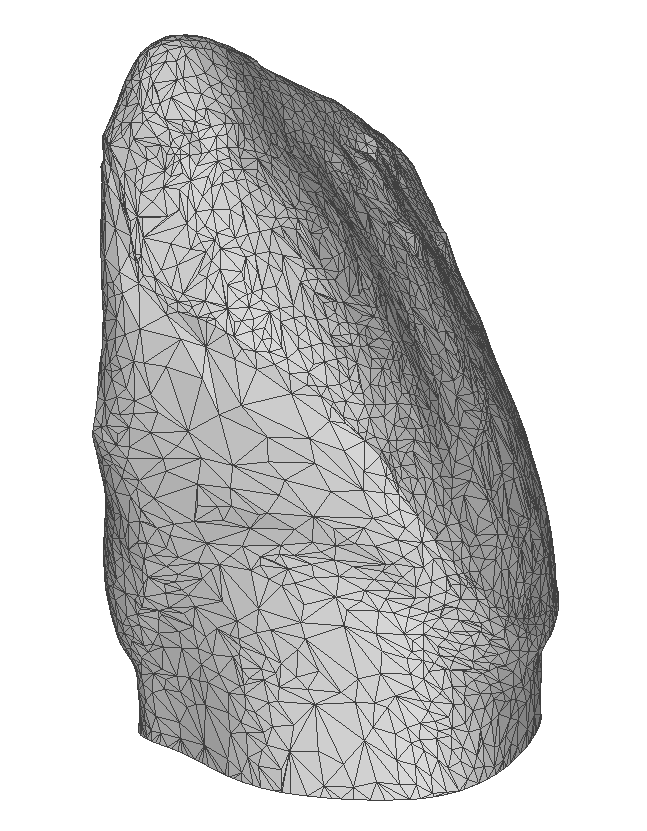
\includegraphics[width=.3\textwidth]{images/snapshot103.png}
    \label{fig:ex1}
    \caption{Примеры данных из выборки в виде трехмерных сеток}
\end{figure*}
\begin{figure*}[ht!]
    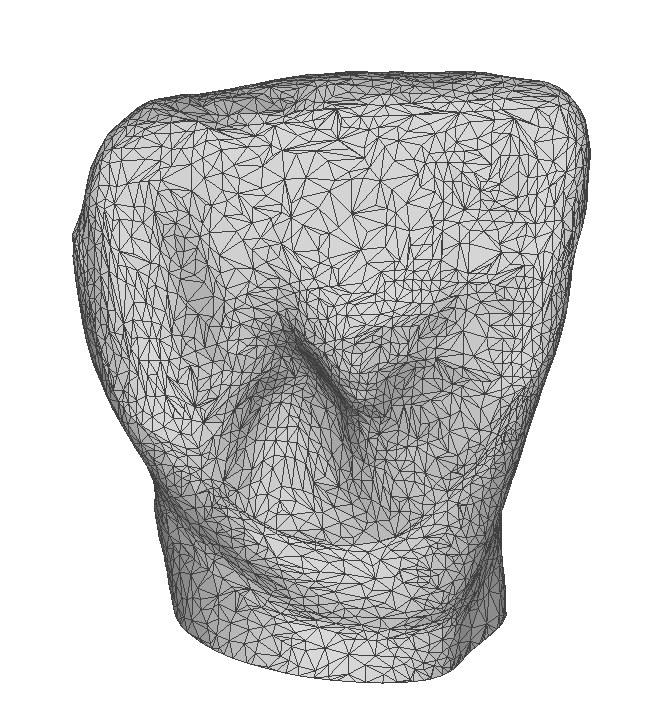
\includegraphics[width=.3\textwidth]{images/snapshot104.png}\hfill
    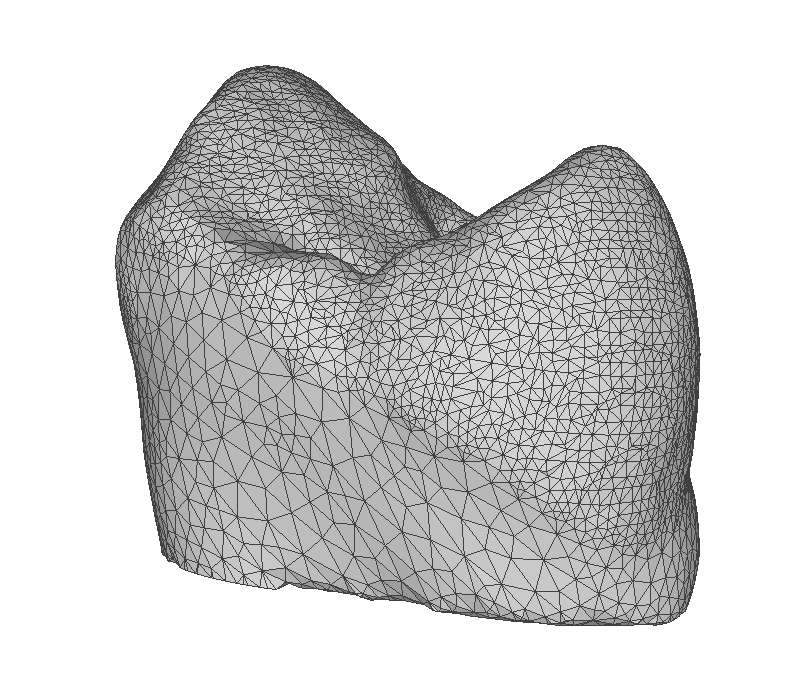
\includegraphics[width=.3\textwidth]{images/snapshot200.png}\hfill
    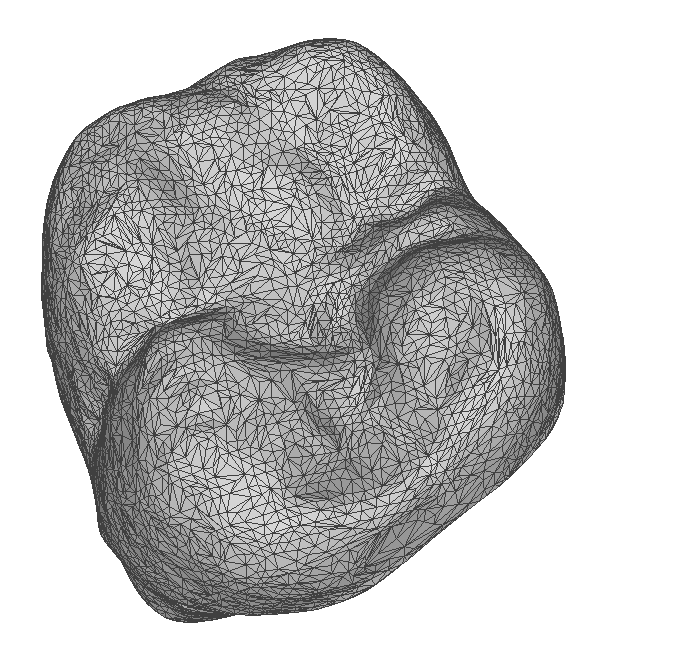
\includegraphics[width=.3\textwidth]{images/snapshot206.png}
    \label{fig:ex2}
    \caption{Примеры данных из выборки в виде трехмерных сеток}
\end{figure*}
\begin{figure*}[ht!]
    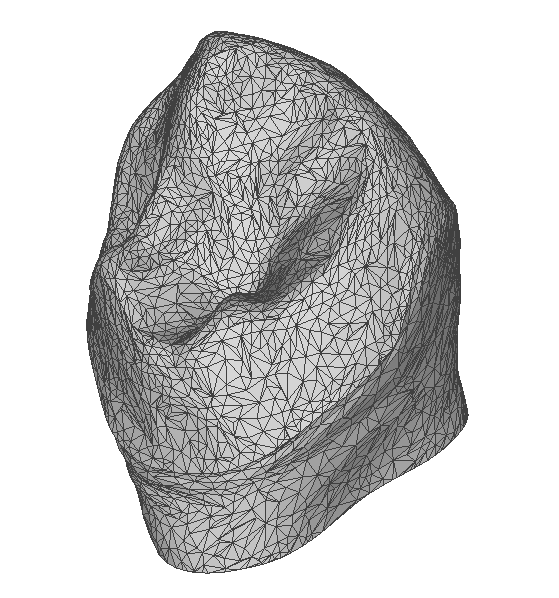
\includegraphics[width=.3\textwidth]{images/snapshot207.png}\hfill
    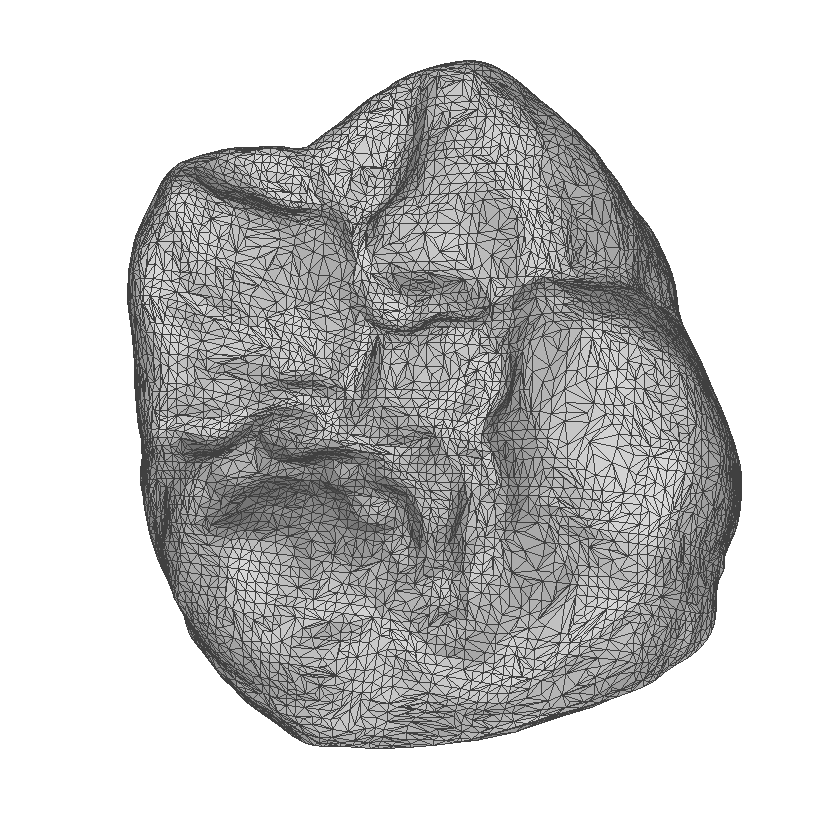
\includegraphics[width=.3\textwidth]{images/snapshot208.png}\hfill
    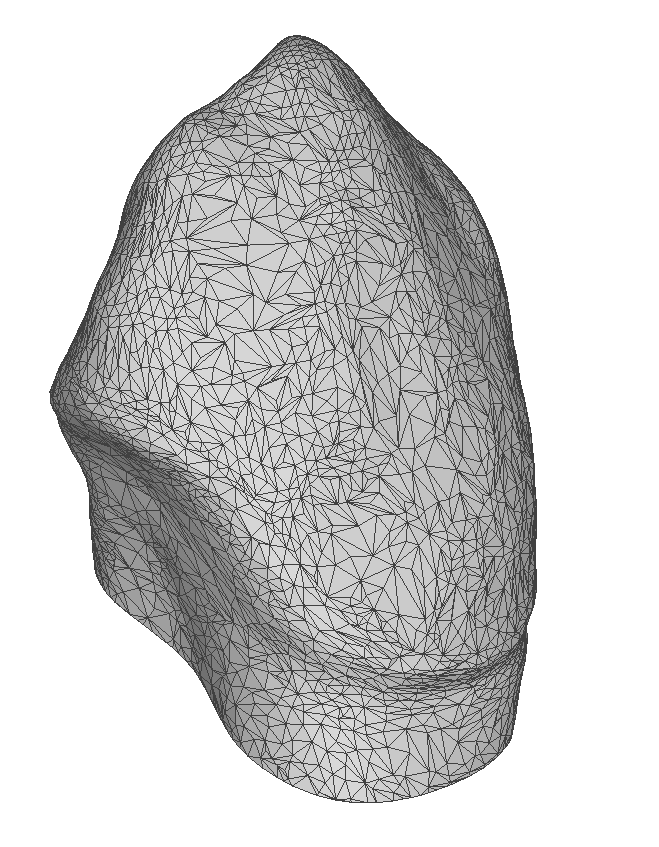
\includegraphics[width=.3\textwidth]{images/snapshot400.png}
    \label{fig:ex3}
    \caption{Примеры данных из выборки в виде трехмерных сеток}
\end{figure*}

\begin{figure*}[ht!]
    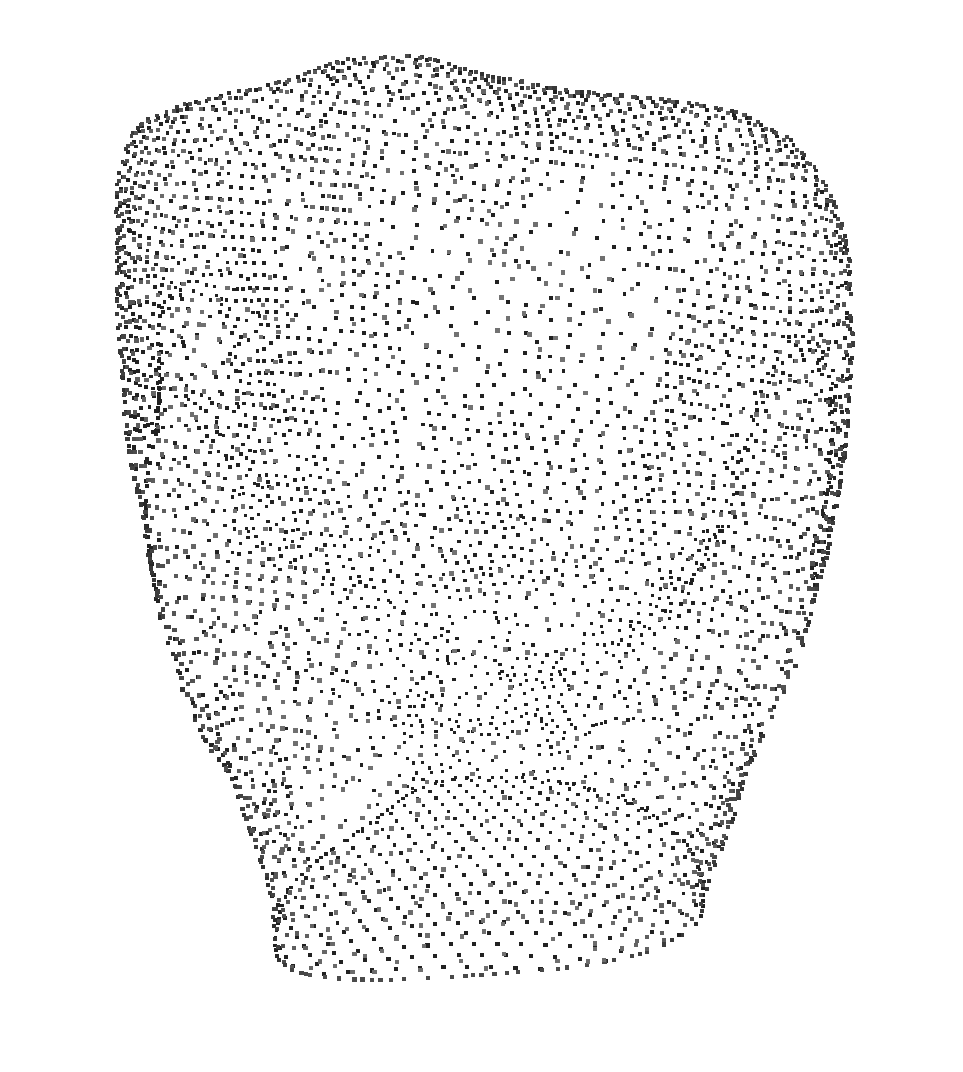
\includegraphics[width=.3\textwidth]{images/snapshot1000.png}\hfill
    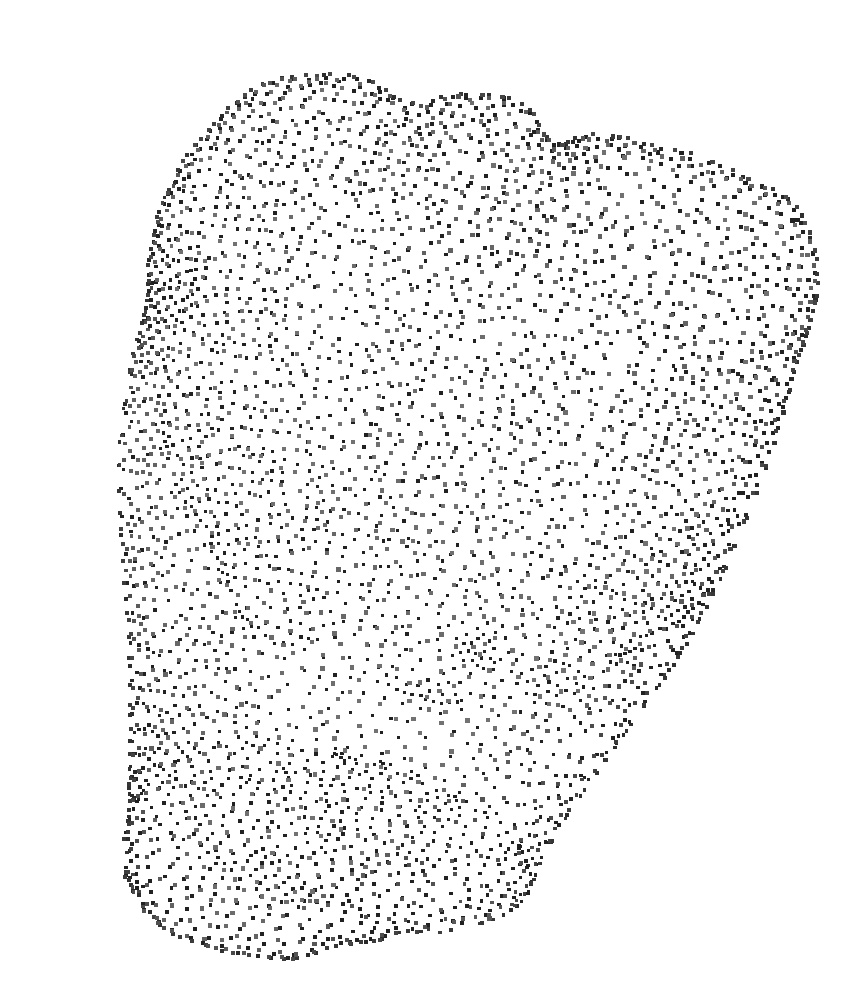
\includegraphics[width=.3\textwidth]{images/snapshot1001.png}\hfill
    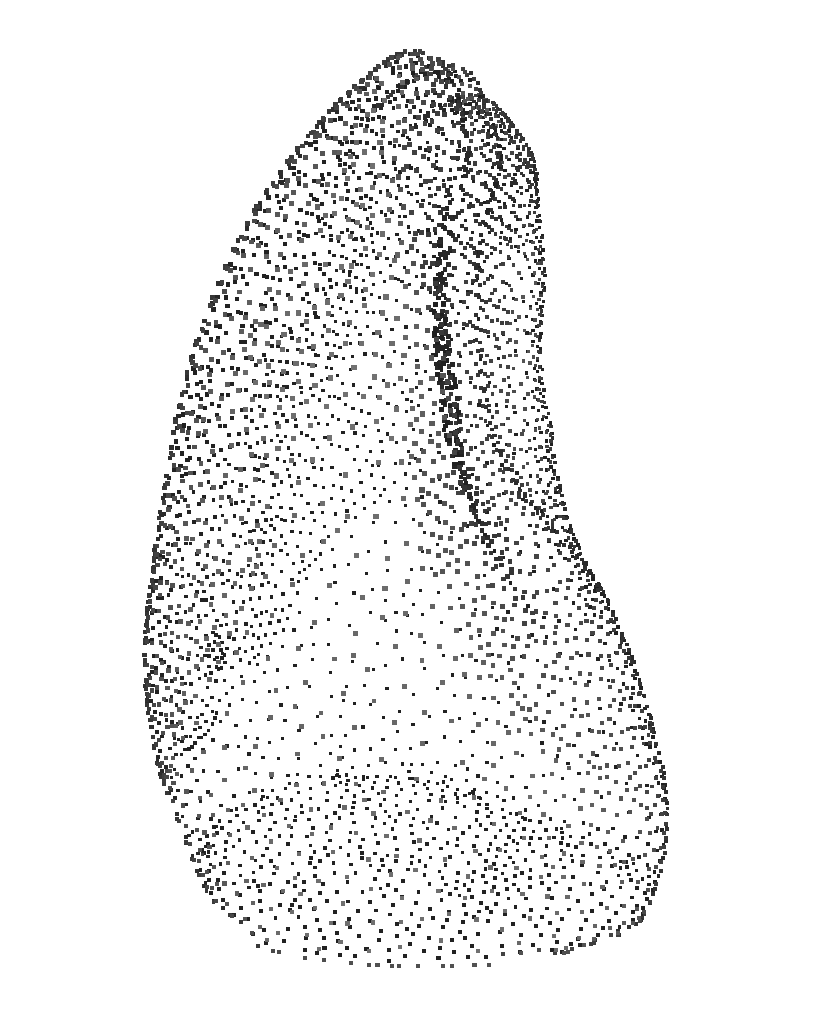
\includegraphics[width=.3\textwidth]{images/snapshot1002.png}
    \label{fig:ex4}
    \caption{Примеры данных из выборки в виде облаков точек}
\end{figure*}
\begin{figure*}[ht!]
    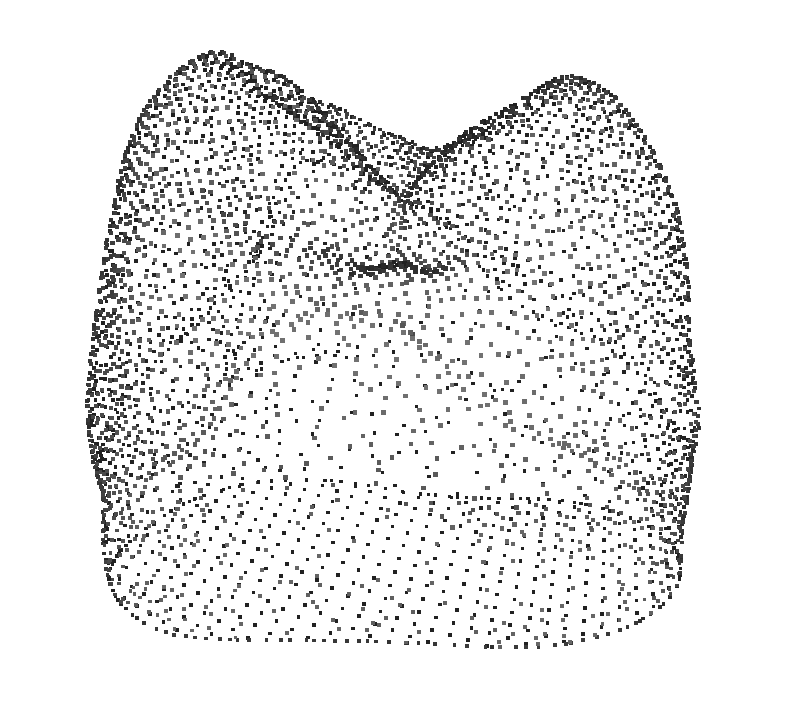
\includegraphics[width=.3\textwidth]{images/snapshot1003.png}\hfill
    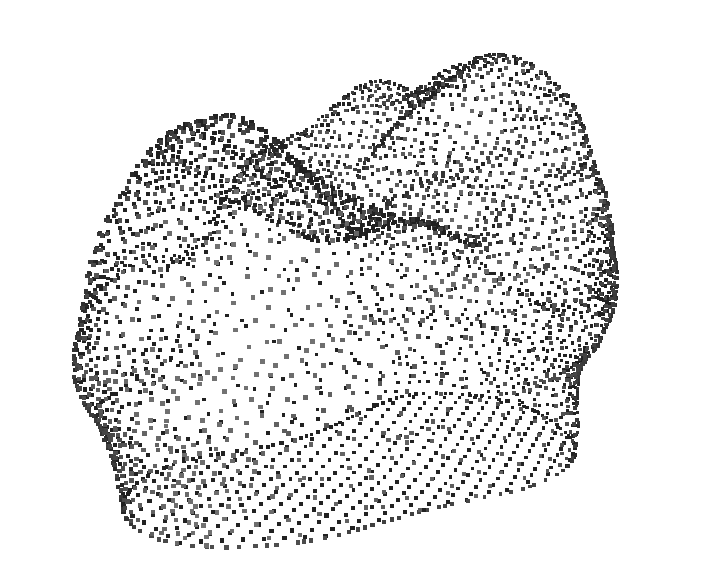
\includegraphics[width=.3\textwidth]{images/snapshot1004.png}\hfill
    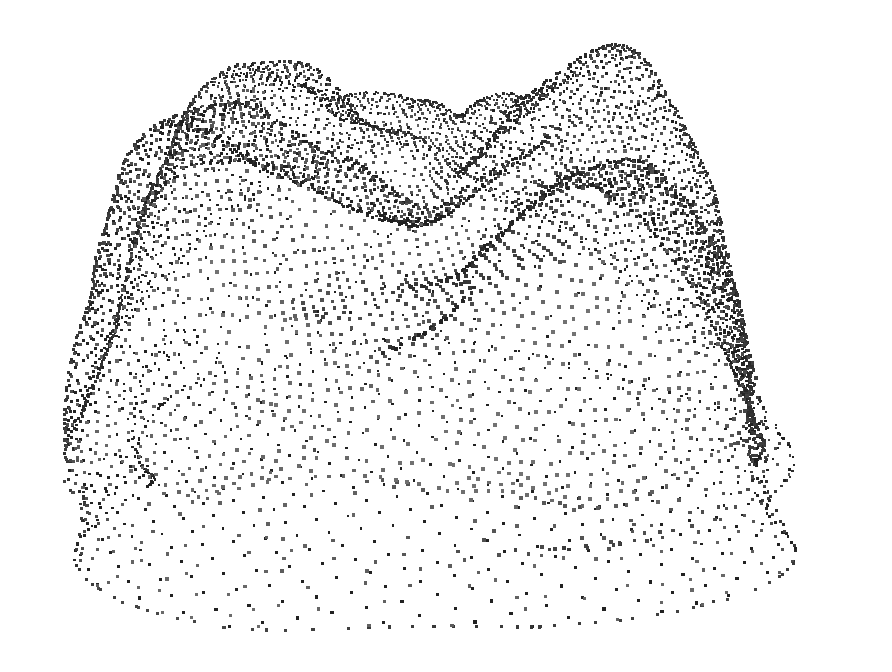
\includegraphics[width=.3\textwidth]{images/snapshot1005.png}
    \label{fig:ex5}
    \caption{Примеры данных из выборки в виде облаков точек}
\end{figure*}
\begin{figure*}[ht!]
    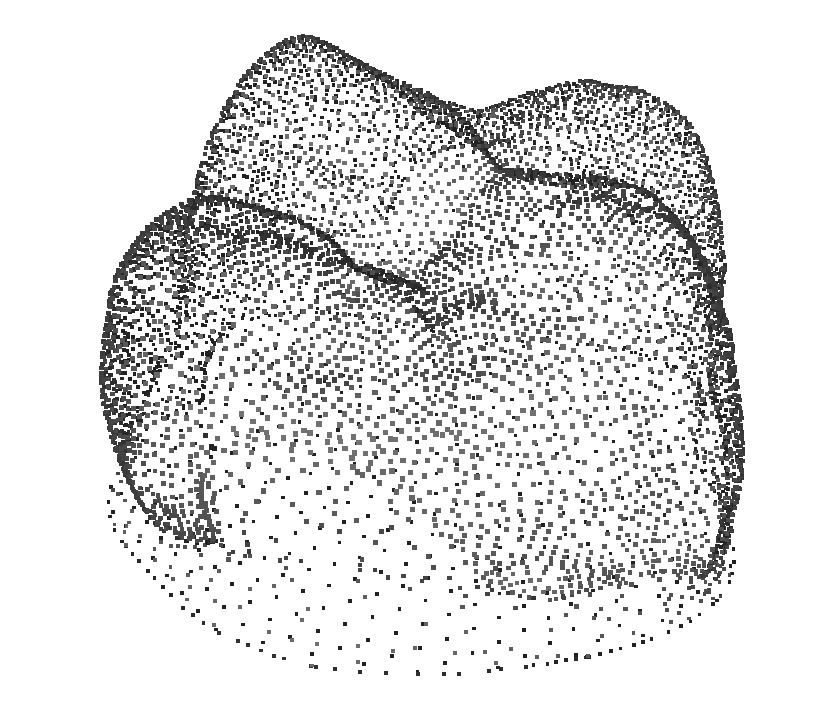
\includegraphics[width=.3\textwidth]{images/snapshot1200.png}\hfill
    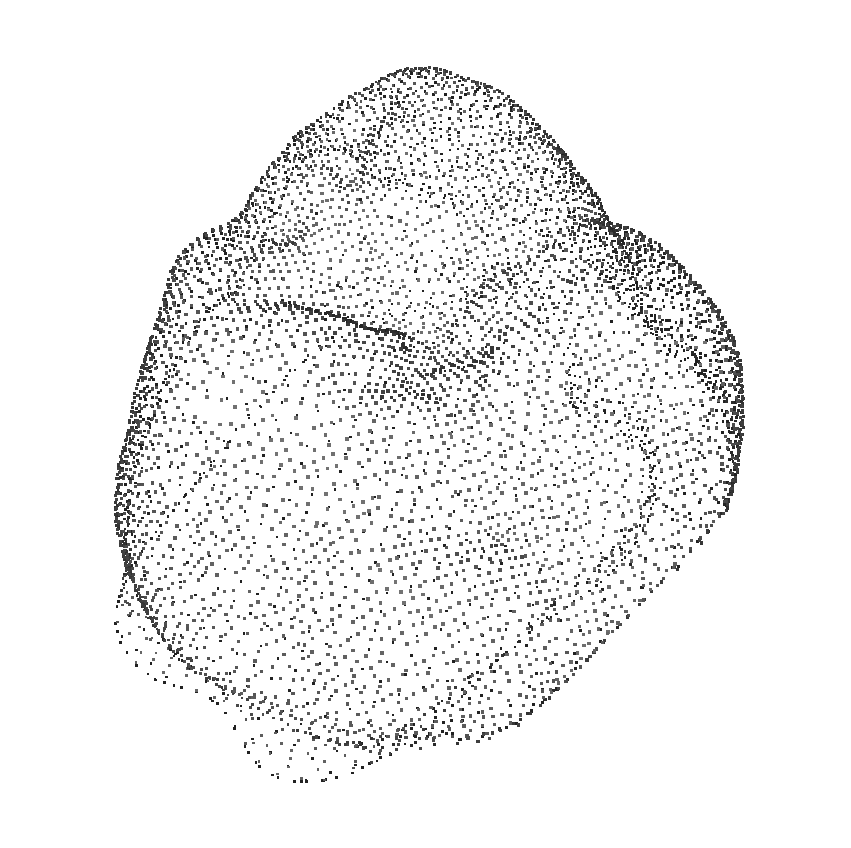
\includegraphics[width=.3\textwidth]{images/snapshot1201.png}\hfill
    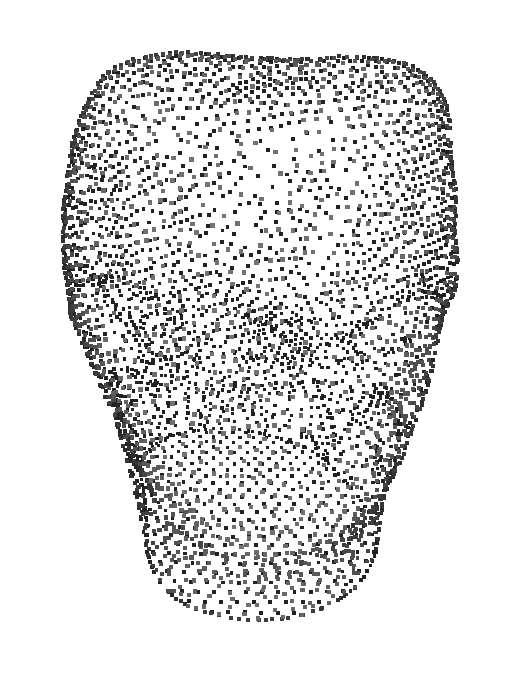
\includegraphics[width=.3\textwidth]{images/snapshot1202.png}
    \label{fig:ex6}
    \caption{Примеры данных из выборки в виде облаков точек}
\end{figure*}